\documentclass{article}
\usepackage{graphicx} % Required for inserting images
\usepackage{geometry}
\usepackage{circuitikz}
\usepackage{siunitx}
\usepackage{CJKutf8}
\usepackage{amsmath}
\usepackage{amssymb}
\usepackage{caption}
\usepackage{float}
\usepackage{subcaption}
\geometry{top=10mm, left=20mm, a4paper}
\title{Frequency Response Report}
\author{梁程捷(B11901136),吳奕娃(B11901080)}
\date{}

\begin{document}
\begin{CJK*}{UTF8}{bkai}
\maketitle

%============Inverting OP-amp====================
\section*{Differential Amplifier with Current-Source Loads}
\begin{minipage}{0.5\textwidth}
\begin{table}[H]
\begin{tabular}{|c|c|c||c|c|c|}
    \hline
    $f$ (\unit{\kilo\hertz}) &  $V_i$ (V)& $V_o$ (V) & $f$ (\unit{\hertz}) &  $V_i$ (V)& $V_o$ (V)\\
    \hline\hline
    1	& 0.400 & 1.24 & 340    & 0.368 & 0.82   \\
    5   & 0.400 & 1.24 & 360    & 0.360 & 0.80  \\
    10	& 0.400 & 1.24 & \textbf{365}& \textbf{0.392} & \textbf{0.86}\\
    50	& 0.384 & 1.22 & 370    & 0.392 & 0.84   \\
    100	& 0.384 & 1.18 & 380    & 0.368 & 0.76   \\
    200	& 0.384 & 1.06 & 400    & 0.336 & 0.68   \\
    300	& 0.368 & 0.90 & 500    & 0.312 & 0.50   \\
    320	& 0.368 & 0.86 &        &      &        \\

\hline
\end{tabular}
\caption{raw experimental data}
\end{table}
\end{minipage}\hspace{20mm}
\begin{minipage}{0.5\textwidth}
    \begin{figure}[H]    
        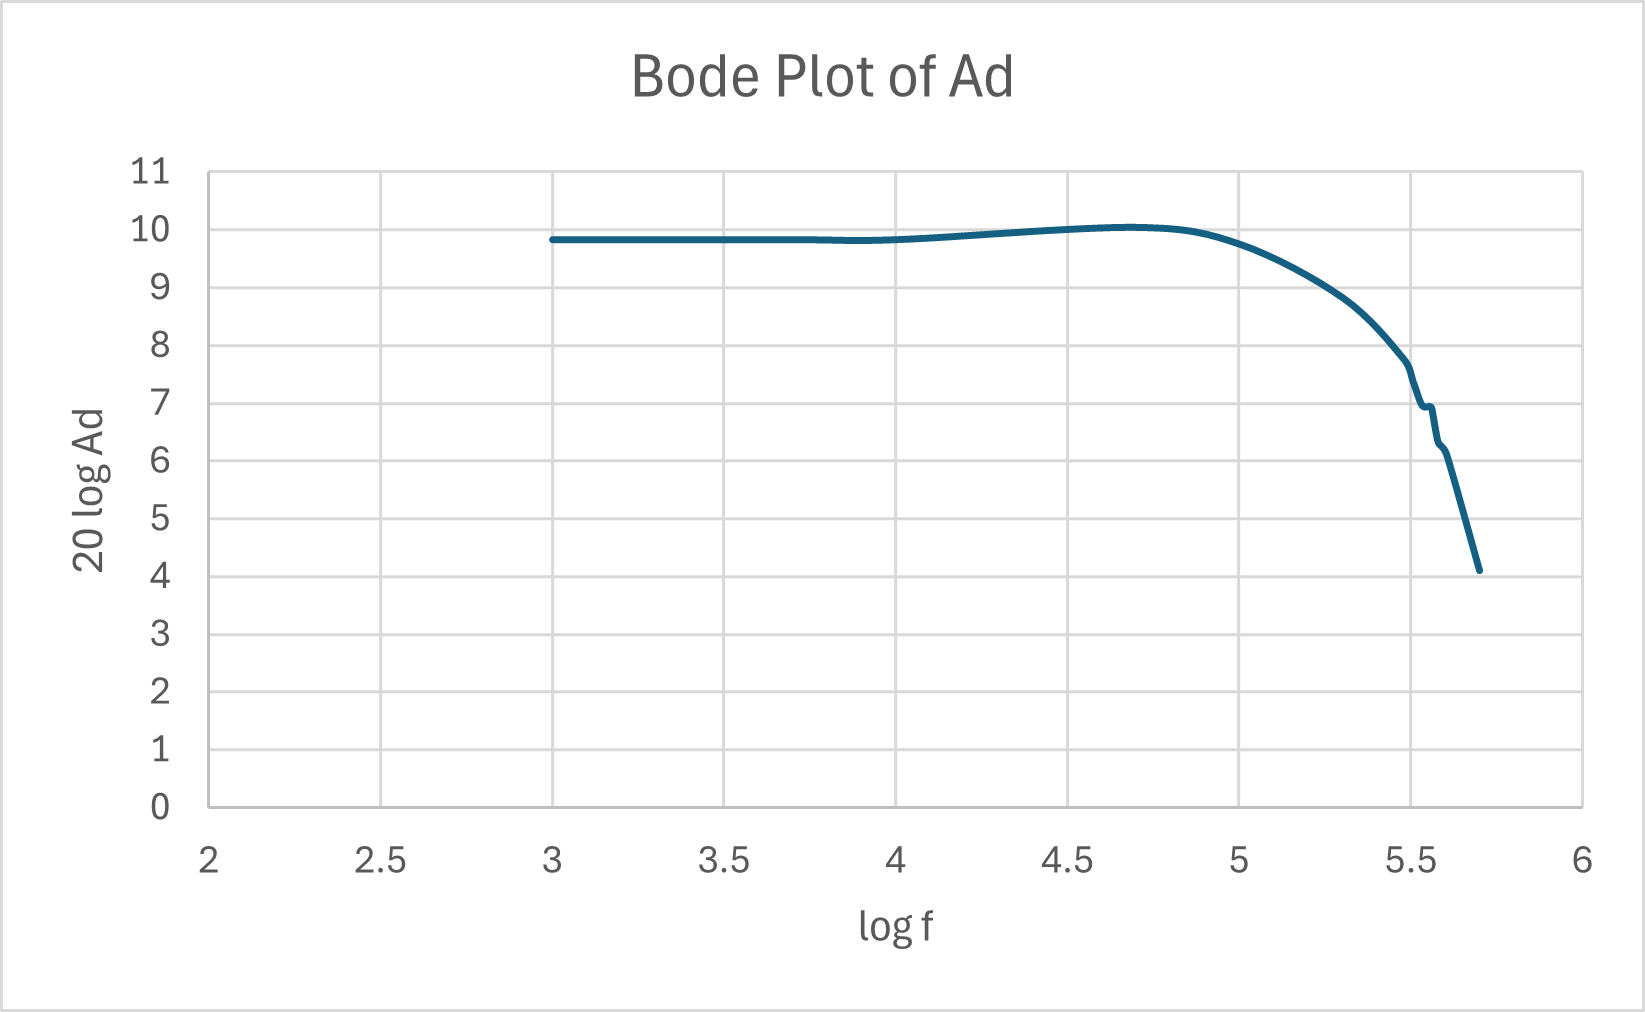
\includegraphics[scale=0.55]{Ad_bode_plot.png}
        \caption{Bode Plot of $A_d$}
    \end{figure}
\end{minipage}
\vspace{3mm}
\textbf{Midband gain $A_M = \frac{1.24}{0.4}$ = 3.1 V/V}, \textbf{$f_{3dB}$ = 365 \unit{\kilo\hertz}}

\section*{Reflections}
\subsection*{梁程捷}
這次實驗我們兩個電路都有做,differential amplifier最後的結果發現是low pass,不是band pass,因爲沒有耦合的大電容,就跟課程一樣。
\subsection*{吳奕娃}
這次的實驗做得還算順利,唯一比較麻煩的地方是在第一個實驗,做低頻率的時候示波器上的訊號不太穩,造成量取數值上的困難。
\end{CJK*}
\end{document}
